\section{Entwurfsphase}
\label{sec:Entwurfsphase}
In der Entwurfsphase sollen aus den Anforderungen der Analysephase Modelle der zu entwickelten Software entstehen, die die konkreten Hardware- und Softwarebezogenen Anforderungen berücksichtigen. Diese Modelle gelten dann als unmittelbare Vorlage für die sich anschließende Implementationsphase. (vgl. \cite[S. 69]{dumke-2003})

Zu Beginn soll eine Marktrecherche durchgeführt werden, um bestehende Lösungen zu analysieren und auf Eignung zu Prüfen. Mit den gewonnen Erkenntnissen soll dann abgewägt werden ob Standartsoftware beschafft wird oder eine eigenentwicklung Veranlasst wird. Das erfolgt im Rahmen einer Variantendiskussion, in der verschiedene Ansätze und Technologien zur Umsetzung der Software bewertet werden.

Letztendlich soll der Programm- und Datenentwurf mithilfe geeigneter Modelle erarbeitet werden. Dies umfasst die Festlegung der Softwarearchitektur, der Datenstruktur sowie etwaiger Schnittstellen und der grafische Oberfläche.

\subsection{Marktrecherche}
\label{sec:Marktrecherche}
%TODO:Schicke Tabelle aus Excel Bauen
Im Rahmen der Marktanalyse wurden drei verschiedene Softwarelösungen für die Anwesenheitsplanung verglichen. Das Ziel dieser Analyse war es, Akquisitionsoptionen für das geplante Softwareprojekt zu ermitteln. Um Entscheidungen über die Eignung treffen zu können, wurden die Softwareprodukte auf den Erfüllungsgrad der Anforderungen geprüft. Dafür wurde eine Bewertungsmatrix erstellt, die funktionale- als auch nichtfunktionale Anforderungen beinhaltete. Dabei wurden die Kriterien so gewählt und gewichtet das zwingend erforderliche Anforderungen höher gewichtet wurden als optionale Anforderungen.

\begin{figure}[htb]
    \centering
    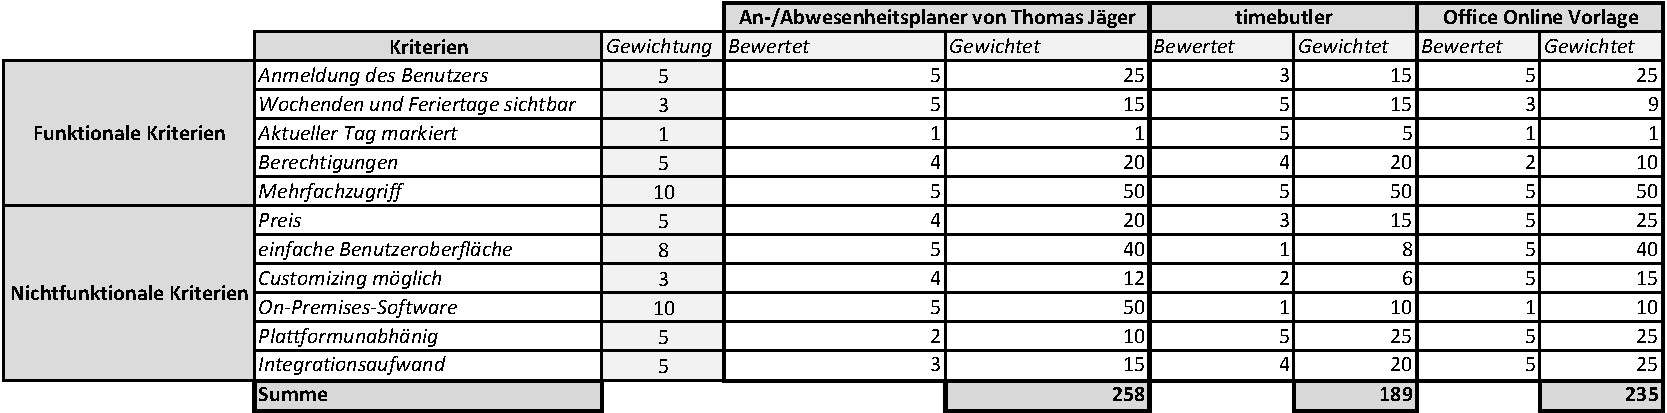
\includegraphics[width=0.9\textwidth,angle=0]{abb/Markterkundung.pdf}
    \caption[Beschreibung]{ Tabelle Markterkundung}
    \label{tab:Markterkundung}
\end{figure}

%TODO:Die Schicke Tabelle hier einfügen!!!
\subsubsection{An-/Abwesenheitsplaner von Thomas Jäger}
\label{sec:AnAbwesenheitsplaner}
Die erste betrachtete Software, der An-/Abwesenheitsplaner von Thomas Jäger, zeichnete sich durch die besonders intuitive Benutzeroberfläche aus. Bei der Betrachtung der anderen funktionalen Kriterien wurde festgestellt, dass die Software alle benötigten Anforderungen erfüllt und damit für den Einsatz geeignet ist. Negativ zu bewerten ist allerding, das die Software nur als Windows Programm zur Verfügung steht und damit nicht Plattformunabhängig eingesetzt werden kann. Zudem müsste ein solches Programm auf jedem Client PC im SMK installiert werden um die Software für alle Nutzbar zu machen. Damit ergibt sich ein hoher initialer Integrationsaufwand und auch späterer Wartungsaufwand den es zu berücksichtigen gilt. (vgl. \cite{AnAbwesenPlaner})


%Die Benutzerfreundlichkeit wurde jedoch als etwas komplex und steil eingestuft, was eine gewisse Einarbeitungszeit erforderte. Zudem war der Support nur eingeschränkt verfügbar und die Preisgestaltung vergleichsweise hoch. (vgl. \cite{AnAbwesenPlaner})
\subsubsection{timebutler}
\label{sec:timebutler}
Das zweite Programm namens timebutler überzeugte hingegen durch seine Plattformunabhängigkeit. Damit könnte es ohne großen Integrationsaufwand im SMK eingeführt und betrieben werden. Die Software bietet alle geforderten Funktionalitäten hat jedoch eine komplizierte Benutzeroberfläche und stellt viele Funktionen bereit die nicht benötigt werden. Das resultiert in höheren Anschaffungskosten als bei dem An-/Abwesenheitsplaner von Thomas Jäger. Besonders negativ ist zu bewerten, dass die Software zwar Plattformunabhängig ist, da sie auf Webtechnologien aufbaut, jedoch nicht als On-Premises-Software verfügbar ist. Damit müsste auf die Cloud des Anbieters zurückgegriffen werden was nicht gewünscht ist. (vgl. \cite{timebutler})

\subsubsection{Online Office Datei}
\label{sec:OnlineOffice}
Die dritte betrachtete Lösung ist die Verwendung einer Online Tabellenkalkulations Vorlage. Das würde es ermöglichen, die bereits vorhandenen Excel Tabellen für die Anwesenheitsplanung weiter zu verwenden. Durch das zurückgreifen auf Online Funktionalitäten die \zB von Microsoft mit Office356 oder mit Onlyoffice in Verbindung mit Nextcloud zur Verfügung stehen, kann man den gleichzeitigen Zugriff auf diese Listern erreichen. Damit würde man das Hauptproblem der einfachen Excel Dateien lösen. Doch auch hier müsste man im Falle des einsatzes von Office356 auf die Microsoft Cloud zurückgreifen. Desweiteren gibt es nur begrenzte Möglichkeit diese Excel Listen vor ungewollter Änderungen zu schützen und ein Berechtigungskonzept durchzusetzten.

\subsubsection{Auswertung der Marktrecherche}
\label{sec:AuswertungMarktrecherche}
Nach Betrachtung der drei Programme wurde festgestellt, dass keines der drei für eine Akquisition in frage kommt, da jedes seine individuellen Schwachstellen mitsich bringt. Der An-/Abwesenheitsplaner von Thomas Jäger wäre von allen die beste Option, da es eine benutzerfreundliche Oberfläche, eine solide Funktionalität und eine angemessene Preisgestaltung vereint. Die Plattformunabhängigkeit ist jedoch im SMK ein großer Faktor, da sich das neue Programm möglichst gut in die vorhandene Infrastruktur einfügen soll. Deswegen wurde sich gegen eine Akquisition von Standartsoftware entschieden. Um die geforderten Funktionalitäten abzubilden ohne dabei die Schwachstellen der Analysierten Programme inkauf nehmen zu müssen wurde ich für eine Eigenentwicklung der Software entschieden.

\subsection{Eigenentwicklung}
\label{sec:Eigenentwicklung}
Referat 12 wurde mit der Entwicklung der Softwarelösung beauftragt. Für die Umsetzung des Projektes werden benötigte Hard- und Softwareressourcen vom SMK bereitgestellt. Um den zeitlichen Rahmen für das Projekt abzugrenzen wurde für das gesamte Projekt 32 Manntage angesetzt. Die genaue Aufschlüsselung des Projektablaufes siehe \ref{abb:Gantt}.

Für die Entwicklung der Software sethen dem Entwickler ein voll ausgestatteter Arbeitsplatz, sowie mehrere virtuelle Maschinen im Rechenzentrum zur Verfügung. Damit hat der Entwickler freie Hand bei der Umsetzung. Zu beachten ist jedoch, dass nach Möglichkeit auf die bestehende Infrastruktur zurückgegriffen bzw. berücksichtigt wird. Da bedeutet das \zB benötigte Datenbanken auf dem bereits vorhandenen SQL Server erstellt werden sollten und keine Entwicklung mit MySql erfolgen sollte, da es im Unternehmen nicht eingesetzt wird.


\subsection{Variantendiskussion}
\label{sec:Marktrecherche}

\subsection{Programm und Datenentwurf}
\label{sec:ProgrammUDatenentwurf}